\documentclass[tikz,border=8pt]{standalone}
% Shared look for every TikZ diagram. Load with \input{../../tools/tikz-style.tex}
\usepackage[T1]{fontenc}
\usepackage{lmodern}
\renewcommand{\sfdefault}{lmr}  % diagrams use the same serif as the text
\usetikzlibrary{arrows.meta, positioning, shapes.geometric, calc, fit, backgrounds}
\definecolor{cblue}{HTML}{4C78A8}
\definecolor{corange}{HTML}{F58518}
\definecolor{cgreen}{HTML}{54A24B}
\definecolor{cred}{HTML}{E45756}
\definecolor{cpurple}{HTML}{B279A2}
\definecolor{cgrey}{HTML}{6B6B6B}
\tikzset{
  every picture/.style={font=\sffamily, line width=1.2pt},
  box/.style={draw=#1, fill=#1!12, rounded corners=4pt, align=center, inner sep=7pt, minimum height=1.1cm},
  box/.default=cgrey,
  arrow/.style={-{Stealth[length=3mm]}, draw=cgrey, line width=1.4pt},
  title/.style={font=\sffamily\bfseries\Large},
  note/.style={font=\sffamily\small, text=cgrey, align=center},
}
\AtBeginDocument{\hyphenpenalty=10000 \exhyphenpenalty=10000}

% The EM algorithm as a loop (MML Section 11.3): initialise; E-step (responsibilities by Bayes' theorem);
% M-step (means, then covariances around the new means, then weights); check the change in log-likelihood.
% Side notes: the seven-observation example, l = -28.33 at the start, -14.41 after one round, -13.973 at convergence.
\begin{document}
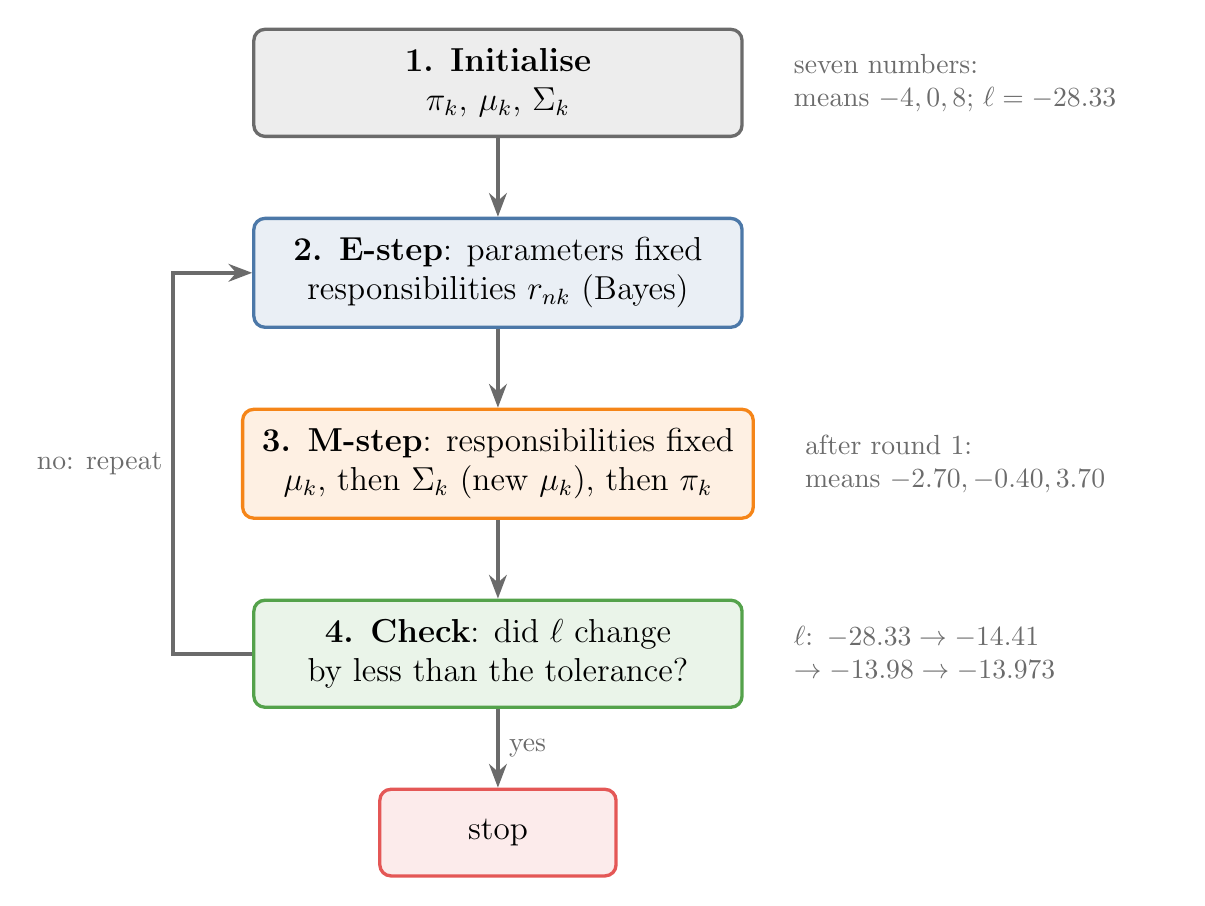
\begin{tikzpicture}[node distance=1.0cm and 1.6cm, every node/.append style={font=\large}]
  \node[box=cgrey, minimum width=6.2cm] (init) {\textbf{1. Initialise}\\ $\pi_k$, $\boldsymbol\mu_k$, $\boldsymbol\Sigma_k$};
  \node[box=cblue, minimum width=6.2cm, below=of init] (e) {\textbf{2. E-step}: parameters fixed\\ responsibilities $r_{nk}$ (Bayes)};
  \node[box=corange, minimum width=6.2cm, below=of e] (m) {\textbf{3. M-step}: responsibilities fixed\\ $\boldsymbol\mu_k$, then $\boldsymbol\Sigma_k$ (new $\boldsymbol\mu_k$), then $\pi_k$};
  \node[box=cgreen, minimum width=6.2cm, below=of m] (c) {\textbf{4. Check}: did $\ell$ change\\ by less than the tolerance?};
  \node[box=cred, minimum width=3cm, below=of c] (stop) {stop};
  \draw[arrow] (init) -- (e);
  \draw[arrow] (e) -- (m);
  \draw[arrow] (m) -- (c);
  \draw[arrow] (c) -- node[right, note, font=\normalsize] {yes} (stop);
  \draw[arrow] (c.west) -- ++(-1.0,0) |- node[pos=0.25, left, note, font=\normalsize] {no: repeat} (e.west);
  \node[note, font=\normalsize, anchor=west, text width=4.6cm, align=left] at ($(init.east)+(0.5,0)$) {seven numbers:\\ means $-4, 0, 8$; $\ell = -28.33$};
  \node[note, font=\normalsize, anchor=west, text width=4.6cm, align=left] at ($(m.east)+(0.5,0)$) {after round 1:\\ means $-2.70, -0.40, 3.70$};
  \node[note, font=\normalsize, anchor=west, text width=4.6cm, align=left] at ($(c.east)+(0.5,0)$) {$\ell$: $-28.33 \to -14.41$\\ $\to -13.98 \to -13.973$};
\end{tikzpicture}
\end{document}
